% Options for packages loaded elsewhere
% Options for packages loaded elsewhere
\PassOptionsToPackage{unicode}{hyperref}
\PassOptionsToPackage{hyphens}{url}
%
\documentclass[
  a4paper,
]{article}
\usepackage{xcolor}
\usepackage[top=20mm,bottom=20mm,left=20mm,right=20mm]{geometry}
\usepackage{amsmath,amssymb}
\setcounter{secnumdepth}{-\maxdimen} % remove section numbering
\usepackage{iftex}
\ifPDFTeX
  \usepackage[T1]{fontenc}
  \usepackage[utf8]{inputenc}
  \usepackage{textcomp} % provide euro and other symbols
\else % if luatex or xetex
  \usepackage{unicode-math} % this also loads fontspec
  \defaultfontfeatures{Scale=MatchLowercase}
  \defaultfontfeatures[\rmfamily]{Ligatures=TeX,Scale=1}
\fi
\usepackage{lmodern}
\ifPDFTeX\else
  % xetex/luatex font selection
\fi
% Use upquote if available, for straight quotes in verbatim environments
\IfFileExists{upquote.sty}{\usepackage{upquote}}{}
\IfFileExists{microtype.sty}{% use microtype if available
  \usepackage[]{microtype}
  \UseMicrotypeSet[protrusion]{basicmath} % disable protrusion for tt fonts
}{}
\makeatletter
\@ifundefined{KOMAClassName}{% if non-KOMA class
  \IfFileExists{parskip.sty}{%
    \usepackage{parskip}
  }{% else
    \setlength{\parindent}{0pt}
    \setlength{\parskip}{6pt plus 2pt minus 1pt}}
}{% if KOMA class
  \KOMAoptions{parskip=half}}
\makeatother
% Make \paragraph and \subparagraph free-standing
\makeatletter
\ifx\paragraph\undefined\else
  \let\oldparagraph\paragraph
  \renewcommand{\paragraph}{
    \@ifstar
      \xxxParagraphStar
      \xxxParagraphNoStar
  }
  \newcommand{\xxxParagraphStar}[1]{\oldparagraph*{#1}\mbox{}}
  \newcommand{\xxxParagraphNoStar}[1]{\oldparagraph{#1}\mbox{}}
\fi
\ifx\subparagraph\undefined\else
  \let\oldsubparagraph\subparagraph
  \renewcommand{\subparagraph}{
    \@ifstar
      \xxxSubParagraphStar
      \xxxSubParagraphNoStar
  }
  \newcommand{\xxxSubParagraphStar}[1]{\oldsubparagraph*{#1}\mbox{}}
  \newcommand{\xxxSubParagraphNoStar}[1]{\oldsubparagraph{#1}\mbox{}}
\fi
\makeatother


\usepackage{longtable,booktabs,array}
\usepackage{calc} % for calculating minipage widths
% Correct order of tables after \paragraph or \subparagraph
\usepackage{etoolbox}
\makeatletter
\patchcmd\longtable{\par}{\if@noskipsec\mbox{}\fi\par}{}{}
\makeatother
% Allow footnotes in longtable head/foot
\IfFileExists{footnotehyper.sty}{\usepackage{footnotehyper}}{\usepackage{footnote}}
\makesavenoteenv{longtable}
\usepackage{graphicx}
\makeatletter
\newsavebox\pandoc@box
\newcommand*\pandocbounded[1]{% scales image to fit in text height/width
  \sbox\pandoc@box{#1}%
  \Gscale@div\@tempa{\textheight}{\dimexpr\ht\pandoc@box+\dp\pandoc@box\relax}%
  \Gscale@div\@tempb{\linewidth}{\wd\pandoc@box}%
  \ifdim\@tempb\p@<\@tempa\p@\let\@tempa\@tempb\fi% select the smaller of both
  \ifdim\@tempa\p@<\p@\scalebox{\@tempa}{\usebox\pandoc@box}%
  \else\usebox{\pandoc@box}%
  \fi%
}
% Set default figure placement to htbp
\def\fps@figure{htbp}
\makeatother





\setlength{\emergencystretch}{3em} % prevent overfull lines

\providecommand{\tightlist}{%
  \setlength{\itemsep}{0pt}\setlength{\parskip}{0pt}}



 


\usepackage{circuitikz}
\usepackage{moresize}
\makeatletter
\@ifpackageloaded{caption}{}{\usepackage{caption}}
\AtBeginDocument{%
\ifdefined\contentsname
  \renewcommand*\contentsname{Table of contents}
\else
  \newcommand\contentsname{Table of contents}
\fi
\ifdefined\listfigurename
  \renewcommand*\listfigurename{List of Figures}
\else
  \newcommand\listfigurename{List of Figures}
\fi
\ifdefined\listtablename
  \renewcommand*\listtablename{List of Tables}
\else
  \newcommand\listtablename{List of Tables}
\fi
\ifdefined\figurename
  \renewcommand*\figurename{Figure}
\else
  \newcommand\figurename{Figure}
\fi
\ifdefined\tablename
  \renewcommand*\tablename{Table}
\else
  \newcommand\tablename{Table}
\fi
}
\@ifpackageloaded{float}{}{\usepackage{float}}
\floatstyle{ruled}
\@ifundefined{c@chapter}{\newfloat{codelisting}{h}{lop}}{\newfloat{codelisting}{h}{lop}[chapter]}
\floatname{codelisting}{Listing}
\newcommand*\listoflistings{\listof{codelisting}{List of Listings}}
\makeatother
\makeatletter
\makeatother
\makeatletter
\@ifpackageloaded{caption}{}{\usepackage{caption}}
\@ifpackageloaded{subcaption}{}{\usepackage{subcaption}}
\makeatother
\usepackage{bookmark}
\IfFileExists{xurl.sty}{\usepackage{xurl}}{} % add URL line breaks if available
\urlstyle{same}
\hypersetup{
  hidelinks,
  pdfcreator={LaTeX via pandoc}}


\author{}
\date{}
\begin{document}


\vspace{20em}

\begin{center}
  \HUGE{{\textbf{Assignment 2}}}
\end{center}

\medskip

\begin{center}
  \large{University of Doha for Science and Technology}
\end{center}

\vspace{50em}

\begin{tabular}{lp{5.0cm}lll}
  &  &  &  & \\
  \textbf{Student Name:} & Fairoos Kunhi

  \  &  &  & \\
  \textbf{Student ID:} & 60315610
  
  \  &  &  & \\
  \textbf{Course Name:} & AETN1112 Digital Electronics
  
  \  &  &  & \\
  \textbf{Section Number:} & 6
  
  \  &  &  & \\
  \textbf{Instructor:} & Premjit Soora
\end{tabular}

\pagenumbering{gobble}

\newpage{}

\pagenumbering{arabic}

\subsection{Part-A}\label{part-a}

\subparagraph{3-26 d}\label{d}

\textbf{Ans:}

\begin{align*}
  \overline{\bar{A} + \overline{(B+C)} + D} \\
  &= \bar{\bar{A}} \cdot \overline{\overline{(B+C)}} \cdot \bar{\bar{D}}
    &\qquad \text{As per DeMorgan's Theorem}\\
  &= A \cdot (B+C) \cdot D
    &\qquad \text{As } \bar{\bar{A}} = A \\
  &= AD \cdot (B+C)
    &\qquad \text{As } AB = BA \\
  &= ADB + ADC
    &\qquad \text{As } A(B+C) = AB + AC \\
\end{align*}

\begin{center}\rule{0.5\linewidth}{0.5pt}\end{center}

\subparagraph{3-29}\label{section}

First, we find the boolean expression of the original circuit:

\begin{figure}

\centering{

\includegraphics[width=3.125in,height=\textheight,keepaspectratio]{assignment2-img/q3-29-circuit.png}

}

\caption{\label{fig-q3-29-circuit}}

\end{figure}%

Unsimplified expression:

\(X = \overline{(\bar{A}+\bar{B})} \cdot BC\)

After simplification, we get: \(\boxed{X = ABC}\)

Gate equivalency table

\begin{longtable}[]{@{}
  >{\raggedright\arraybackslash}p{(\linewidth - 2\tabcolsep) * \real{0.5000}}
  >{\raggedright\arraybackslash}p{(\linewidth - 2\tabcolsep) * \real{0.5000}}@{}}
\toprule\noalign{}
\begin{minipage}[b]{\linewidth}\raggedright
Gate
\end{minipage} & \begin{minipage}[b]{\linewidth}\raggedright
Equivalent NOR gate circuit
\end{minipage} \\
\midrule\noalign{}
\endhead
\bottomrule\noalign{}
\endlastfoot
1 input NOT gate &
\includegraphics[width=3.125in,height=\textheight,keepaspectratio]{assignment2-img/not-output-type-nor-circuit.png} \\
3 input AND gate &
\includegraphics[width=3.125in,height=\textheight,keepaspectratio]{assignment2-img/and-output-type-nor-circuit.png} \\
2 input OR gate &
\includegraphics[width=3.125in,height=\textheight,keepaspectratio]{./assignment2-img/or-output-type-nor-circuit.png} \\
\end{longtable}

With these defined, we replace the original circuit's gates with their
equivalents. Then we get the following circuit:

\begin{figure}

\centering{

\includegraphics[width=6.25in,height=\textheight,keepaspectratio]{./assignment2-img/q29-resultant-circuit.png}

}

\caption{\label{fig-q29-resultant-circuit}}

\end{figure}%

The resultant boolean expression of this is:

\[\overline{\overline{\overline{\left(\overline{\overline{\overline{\overline{\overline{A}+\overline{B}}}}}+\overline{B}\right)}}+\overline{C}}\]

Here's the simplification process:

\begin{align*}
X =\overline{\overline{\overline{\left(\overline{\overline{\overline{\overline{\overline{A}+\overline{B}}}}}+\overline{B}\right)}}+\overline{C}} \\
  &= \overline{{\overline{{\overline{{\overline{{\overline{{\overline{{A}}}+{\overline{{B}}}}}}}}}}}+{\overline{{B}}}+\overline{C}}
    &\qquad \text{As } \bar{\bar{A}} = A \\
  &= \overline{{\overline{{\overline{{\overline{{A}}}+{\overline{{B}}}}}}}+\overline{B}+\overline{C}}
    &\qquad \text{As } \bar{\bar{A}} = A \\
  &= \overline{{\overline{{A}}}+{\overline{{B}}}+{\overline{{B}}}+{\overline{{C}}}}
    &\qquad \text{As } \bar{\bar{A}} = A \\
  &= {\overline{{\overline{{A}}}}}\ {\overline{{\overline{{B}}}}}\ {\overline{{\overline{{B}}}}}\ {\overline{{\overline{{C}}}}}
    &\qquad \text{As per DeMorgan's Theorem} \\
  &= A{B}{B}{C}
    &\qquad \text{As } \bar{\bar{A}} = A \\
  &= \boxed{A{B}C}
    &\qquad \text{As } AA = A \\
\end{align*}

And so, we have found that the original circuit and the new circuit are
both equivalent.

\begin{center}\rule{0.5\linewidth}{0.5pt}\end{center}

\subparagraph{3-33}\label{section-1}

a)

Engine turns on in any of the following cases:

\begin{itemize}
\tightlist
\item
  The button on trunk lid is pressed and the engine is off OR
\item
  The engine is off, the car is unlocked and the button on trunk lid is
  pressed OR
\item
  The engine is on, the car is unlocked, the button on trunk lid is
  pressed and the parking brakes are set
\end{itemize}

b)

\(\mathrm{Trunk\_unlock = (FOB \cdot \overline{Motor\_on}) + (\overline{Motor\_on} \cdot \overline{Locked} \cdot LID) + (Motor\_on \cdot \overline{Locked} \cdot LID \cdot PBrake)}\)

c)

\begin{longtable}[]{@{}ll@{}}
\toprule\noalign{}
Original Value & Equivalent Letter \\
\midrule\noalign{}
\endhead
\bottomrule\noalign{}
\endlastfoot
LID & A \\
FOB & B \\
Locked & C \\
PBrake & D \\
Motor\_on & E \\
\end{longtable}

With theses substitutions, the circuit is labelled as below:

\includegraphics[width=3.125in,height=\textheight,keepaspectratio]{./assignment2-img/q3-33-question-circuit.png}

\begin{longtable}[]{@{}
  >{\raggedright\arraybackslash}p{(\linewidth - 2\tabcolsep) * \real{0.5000}}
  >{\raggedright\arraybackslash}p{(\linewidth - 2\tabcolsep) * \real{0.5000}}@{}}
\toprule\noalign{}
\begin{minipage}[b]{\linewidth}\raggedright
Gate
\end{minipage} & \begin{minipage}[b]{\linewidth}\raggedright
Equivalent NAND gate circuit
\end{minipage} \\
\midrule\noalign{}
\endhead
\bottomrule\noalign{}
\endlastfoot
1 input NOT gate &
\includegraphics[width=3.125in,height=\textheight,keepaspectratio]{./assignment2-img/2nand-as-not.png} \\
2 input AND gate &
\includegraphics[width=3.125in,height=\textheight,keepaspectratio]{./assignment2-img/2nand-as-2and.png} \\
3 input OR gate &
\includegraphics[width=3.125in,height=\textheight,keepaspectratio]{./assignment2-img/2-3nand-as-3or.png} \\
3 input AND gate &
\pandocbounded{\includegraphics[keepaspectratio]{./assignment2-img/3nand-as-3and.png}} \\
4 input AND gate &
\pandocbounded{\includegraphics[keepaspectratio]{./assignment2-img/4nand-as-4and.png}} \\
\end{longtable}

With the above table, from the figure 3-57, we get the following NAND
only circuit:

\includegraphics[width=3.125in,height=\textheight,keepaspectratio]{./assignment2-img/q3-33-resultant-circuit.png}

After simplifying,

\(X = A\bar{B}+\bar{B}\bar{C}D +D\bar{C}DE\)

\newpage{}

\subparagraph{3-40}\label{section-2}

After simplification:

\(X = (\bar{A}\cdot B) BC +\bar{D}+E\)

Therefore, only 1 input, E, is needed. It should have input 1.

\begin{center}\rule{0.5\linewidth}{0.5pt}\end{center}

4-1. Simplify the following expressions using Boolean algebra.

\begin{enumerate}
\def\labelenumi{(\alph{enumi})}
\setcounter{enumi}{1}
\tightlist
\item
  \(y=(Q+R)(\overline{Q}+\overline{R})\)
\end{enumerate}

\textbf{Ans:}

\begin{align*}
  y=(Q+R)(\overline{Q}+\overline{R}) \\
  &= (\overline{Q}+\overline{R})Q+(\bar{Q}+\overline{R})R
    &\qquad \text{Distribution} \\
  &= \overline{Q}Q+Q\overline{R}+R\overline{Q}+{R}{\overline{R}}
    &\qquad \text{Distribution} \\
  &= 0+Q\overline{R}+R\overline{Q}+{R}{\overline{R}}
    &\qquad \text{As } A\bar{A} = 0 \\
  &= 0+Q\overline{R}+R\overline{Q}+0
    &\qquad \text{As } A\bar{A} = 0 \\
  &= \boxed{Q\overline{R}+R\overline{Q}}
    &\qquad \text{As } A+0 = A \\
\end{align*}

\begin{enumerate}
\def\labelenumi{(\alph{enumi})}
\setcounter{enumi}{3}
\tightlist
\item
  \(q=\overline{RST}(\overline{R+S+T})\)
\end{enumerate}

\textbf{Ans:}

\begin{align*}
  q = \overline{RST} (\overline{R + S + T})\\
  &= (\overline{R} + \overline{S} + \overline{T}) \overline{R + S + T}
    &\qquad \text{As per DeMorgan's Theorem}\\
  &= (\overline{R} + \overline{S} + \overline{T}) \overline{R} \ \overline{S} \ \overline{T}
    &\qquad \text{As per DeMorgan's Theorem}\\
  &= \overline{R}\  \overline{S}\  \overline{T}\  \overline{R}\  + \overline{R}\  \overline{S}\  \overline{T}\  \overline{S}\  + \overline{R}\  \overline{S}\  \overline{T}\  \overline{T}
    &\ \text{Distribution} \\
  &= \overline{R}\  \overline{S}\  \overline{T}\ + \overline{R}\  \overline{S}\  \overline{T}\ + \overline{R}\  \overline{S}\  \overline{T}
    &\qquad \text{As } AA = A \\
  &= \boxed{\overline{R}\  \overline{S}\  \overline{T}}
    &\qquad \text{As } AA = A \\
\end{align*}

\begin{enumerate}
\def\labelenumi{(\alph{enumi})}
\setcounter{enumi}{7}
\tightlist
\item
  \(x=AB(\overline{\overline{C}D})+\overline{A}BD+\overline{B}\overline{C}\overline{D}\)
\end{enumerate}

\textbf{Ans:}

\begin{align*}
  x=AB(\overline{\overline{C}D})+\overline{A}BD+\overline{B}\overline{C}\overline{D} \\
  &= AB({\overline{{\overline{{C}}}}}+{\overline{{D}}})+\overline{A}BD+\overline{B}\ \overline{C}\ \overline{D}
    &\qquad \text{As per DeMorgan's Theorem}\\
  &= AB({C}+\overline{D})+\overline{A}BD+\overline{B}\ \overline{C}\ \overline{D}
    &\qquad \text{As } \bar{\bar{A}} = A \\
  &= \boxed{ABC+AB\overline{D}+\overline{A}BD+\overline{B}\ \overline{C}\ \overline{D}}
    &\qquad \text{Distribution} \\
\end{align*}

\begin{center}\rule{0.5\linewidth}{0.5pt}\end{center}

\subparagraph{4.11. Determine the minimum expression for each K
map}\label{determine-the-minimum-expression-for-each-k-map}

\begin{enumerate}
\def\labelenumi{\alph{enumi}.}
\tightlist
\item
\end{enumerate}

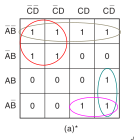
\includegraphics[width=3.125in,height=\textheight,keepaspectratio]{assignment2_files/mediabag/assignment2-img/4-11-a.pdf}

\(X = \bar{A}\bar{C} + \bar{B}C + ABC\bar{D}\)

\begin{enumerate}
\def\labelenumi{\alph{enumi}.}
\setcounter{enumi}{1}
\tightlist
\item
\end{enumerate}

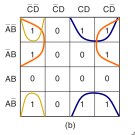
\includegraphics[width=3.125in,height=\textheight,keepaspectratio]{assignment2_files/mediabag/assignment2-img/q4-11-b.pdf}

\(X = A\bar{B}\bar{D}\)

\newpage{}

\begin{enumerate}
\def\labelenumi{\alph{enumi}.}
\setcounter{enumi}{2}
\tightlist
\item
\end{enumerate}

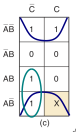
\includegraphics[width=1.04167in,height=\textheight,keepaspectratio]{assignment2_files/mediabag/assignment2-img/q4-11-c.pdf}

X = \bar\{A\}\bar\{B\} + A\bar\{C\}

\begin{center}\rule{0.5\linewidth}{0.5pt}\end{center}

\subparagraph{4-17.}\label{section-3}

\begin{longtable}[]{@{}ll@{}}
\toprule\noalign{}
Original Value & Equivalent Letter \\
\midrule\noalign{}
\endhead
\bottomrule\noalign{}
\endlastfoot
SW1 & A \\
SW2 & B \\
SW3 & C \\
SW4 & D \\
\end{longtable}

We shall assume that:

\begin{itemize}
\tightlist
\item
  Closed switch = input 0
\item
  Open switch = input 1
\end{itemize}

Then we get the following truth table:

\begin{enumerate}
\def\labelenumi{\arabic{enumi}.}
\tightlist
\item
  \& 2. answers
\end{enumerate}

\begin{longtable}[]{@{}
  >{\centering\arraybackslash}p{(\linewidth - 12\tabcolsep) * \real{0.1549}}
  >{\centering\arraybackslash}p{(\linewidth - 12\tabcolsep) * \real{0.0704}}
  >{\centering\arraybackslash}p{(\linewidth - 12\tabcolsep) * \real{0.0704}}
  >{\centering\arraybackslash}p{(\linewidth - 12\tabcolsep) * \real{0.0704}}
  >{\centering\arraybackslash}p{(\linewidth - 12\tabcolsep) * \real{0.0704}}
  >{\centering\arraybackslash}p{(\linewidth - 12\tabcolsep) * \real{0.0704}}
  >{\raggedright\arraybackslash}p{(\linewidth - 12\tabcolsep) * \real{0.4930}}@{}}
\toprule\noalign{}
\begin{minipage}[b]{\linewidth}\centering
Decimal equivalent
\end{minipage} & \begin{minipage}[b]{\linewidth}\centering
A
\end{minipage} & \begin{minipage}[b]{\linewidth}\centering
B
\end{minipage} & \begin{minipage}[b]{\linewidth}\centering
C
\end{minipage} & \begin{minipage}[b]{\linewidth}\centering
D
\end{minipage} & \begin{minipage}[b]{\linewidth}\centering
X
\end{minipage} & \begin{minipage}[b]{\linewidth}\raggedright
Expression for X
\end{minipage} \\
\midrule\noalign{}
\endhead
\bottomrule\noalign{}
\endlastfoot
0 & 0 & 0 & 0 & 0 & X & \\
1 & 0 & 0 & 0 & 1 & 1 & \(m_{1}=A\bar{B}\bar{C}\bar{D}\) \\
2 & 0 & 0 & 1 & 0 & X & \\
3 & 0 & 0 & 1 & 1 & 1 & \(m_{3} = AB\bar{C}\bar{D}\) \\
4 & 0 & 1 & 0 & 0 & X & \\
5 & 0 & 1 & 0 & 1 & 1 & \(m_5=A\bar{B}C\bar{D}\) \\
6 & 0 & 1 & 1 & 0 & X & \\
7 & 0 & 1 & 1 & 1 & 0 & \\
8 & 1 & 0 & 0 & 0 & 1 & \(m_8=\bar{A}\bar{B}\bar{C}D\) \\
9 & 1 & 0 & 0 & 1 & 1 & \(m_9=A\bar{B}\bar{C}D\) \\
10 & 1 & 0 & 1 & 0 & 1 & \(m_{ 10 }=\bar{A}B\bar{C}D\) \\
11 & 1 & 0 & 1 & 1 & 0 & \\
12 & 1 & 1 & 0 & 0 & 1 & \(m_{12}=\bar{A}\bar{B}CD\) \\
13 & 1 & 1 & 0 & 1 & 0 & \\
14 & 1 & 1 & 1 & 0 & 0 & \\
15 & 1 & 1 & 1 & 1 & 0 & \\
\end{longtable}

\begin{enumerate}
\def\labelenumi{\arabic{enumi}.}
\setcounter{enumi}{2}
\item
  \(X = \sum m (3, 5, 6, 7, 10, 12, 14)\)
\item
  \(X = \bar{A}\bar{B}CD + \bar{A}B\bar{C}D + \bar{A}BC\bar{D} + \bar{A}BCD + A\bar{B}C\bar{D} + AB\bar{C}\bar{D} + ABC\bar{D}\)
\item
  K-map is given below:
\end{enumerate}

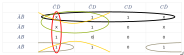
\includegraphics[width=4.16667in,height=\textheight,keepaspectratio]{assignment2_files/mediabag/assignment2-img/q4-17-k-map.pdf}

\begin{enumerate}
\def\labelenumi{\arabic{enumi}.}
\setcounter{enumi}{5}
\tightlist
\item
  \(X = \bar{A}CD + AB \bar{D} + \bar{A}D + BC + AC\)
\end{enumerate}

\newpage{}

\subsection{Part-B}\label{part-b}

\subparagraph{1. For the below truth table answer the related questions
that
follow.}\label{for-the-below-truth-table-answer-the-related-questions-that-follow.}

\begin{figure}

\centering{

\includegraphics[width=3.125in,height=\textheight,keepaspectratio]{assignment2-img/part-b-q1-truth-table.png}

}

\caption{\label{fig-part-b-q1-truth-table}}

\end{figure}%

a) Write the Maxterms.

\textbf{Ans:}

Maxterms: \((A+B+C), (A+B+\bar{C}), (A+\bar{B}+C), (\bar{A}+B+C)\)

b) Extract the canonical Boolean expression using POS

\textbf{Ans:}

POS: \((A+B+C) + (A+B+\bar{C}) + (A+\bar{B}+C) + (\bar{A}+B+C)\)

\begin{center}\rule{0.5\linewidth}{0.5pt}\end{center}

\subparagraph{2. Convert the following numbers using the weighted
method}\label{convert-the-following-numbers-using-the-weighted-method}

2.(a) Binary ➜ Decimal

(i) \(11001101\)

\[
\begin{matrix}
7 & 6 & 5 & 4 & 3 & 2 & 1 & 0 \\
1 & 1 & 0 & 0 & 1 & 1 & 0 & 1 \\
\end{matrix}
\]

\begin{align*}
1\cdot 2^7 &+ 1\cdot 2^6 + 0\cdot 2^5 + 0\cdot 2^4 + 1\cdot 2^3 + 1\cdot 2^2 + 0\cdot 2^1 + 1\cdot 2^0 \\
&= 128 + 64 + 0 + 0 + 8 + 4 + 0 + 1 \\
&= \boxed{(205)_{10}}
\end{align*}

(ii) \(00111110\)

\[
\begin{matrix}
7 & 6 & 5 & 4 & 3 & 2 & 1 & 0 \\
0 & 0 & 1 & 1 & 1 & 1 & 1 & 0 \\
\end{matrix}
\]

\begin{align*}
0\cdot 2^7 &+ 0\cdot 2^6 + 1\cdot 2^5 + 1\cdot 2^4 + 1\cdot 2^3 + 1\cdot 2^2 + 1\cdot 2^1 + 0\cdot 2^0 \\
&= 0 + 0 + 32 + 16 + 8 + 4 + 2 + 0 \\
&= \boxed{(62)_{10}}
\end{align*}

\begin{center}\rule{0.5\linewidth}{0.5pt}\end{center}

2.(b) Decimal ➜ Binary

(i) \((168)_{10}\)

\[
\begin{matrix}
7 & 6 & 5 & 4 & 3 & 2 & 1 & 0 \\
1 & 0 & 1 & 0 & 1 & 0 & 0 & 0 \\
\end{matrix}
\]

\begin{align*}
168 &= 1\cdot 2^7 + 0\cdot 2^6 + 1\cdot 2^5 + 0\cdot 2^4 + 1\cdot 2^3 + 0\cdot 2^2 + 0\cdot 2^1 + 0\cdot 2^0 \\
&= 128 + 0 + 32 + 0 + 8 + 0 + 0 + 0 \\
&= \boxed{(10101000)_2}
\end{align*}

\textbf{(ii)} \((216)_{10}\)

\[
\begin{matrix}
7 & 6 & 5 & 4 & 3 & 2 & 1 & 0 \\
1 & 1 & 0 & 1 & 1 & 0 & 0 & 0 \\
\end{matrix}
\]

\begin{align*}
216 &= 1\cdot 2^7 + 1\cdot 2^6 + 0\cdot 2^5 + 1\cdot 2^4 + 1\cdot 2^3 + 0\cdot 2^2 + 0\cdot 2^1 + 0\cdot 2^0 \\
&= 128 + 64 + 0 + 16 + 8 + 0 + 0 + 0 \\
&= \boxed{(11011000)_2}
\end{align*}




\end{document}
